%! Author = matteomagnini
%! Date = 03/03/26

% Preamble
\documentclass[11pt]{article}

% Packages
\usepackage{amsmath}
\usepackage{amssymb}
\usepackage{tikz}
\usepackage{hyperref}
\usetikzlibrary{positioning}

\title{
    Intelligent Systems 2\\
    Tutorial week 3: Modal Logic
}

\author{
    Matteo Magnini\\
    \href{mailto:matteo.magnini@uni.lu}{matteo.magnini@uni.lu}
}

\date{
    5 March, 2026
}

% Document
\begin{document}

    \maketitle

    \section{Solutions}

    \subsection{Exercise 1}

    Which of the following statements are true?
    Explain your answer.
    \begin{enumerate}
        \item[(a)] $M, s_1 \models p$\\
        \textbf{True.} $p$ is in the valuation for $s_1$.

        \item[(b)] $M, s_1 \models \Box q$\\
        \textbf{True.} $\Box q$ means ``in all successors of $s_1$, $q$ is true.''
        $s_1$ has two successors: $s_2$ (where $q$ is true), $s_4$ (where $q$ is true).
        So, $q$ is true in both successors, so $M, s_1 \models \Box q$ is \textbf{True}.

        \item[(c)] $M, s_2 \models q \wedge \Box q$\\
        \textbf{False.} $q$ is true in $s_2$, but $\Box q$ means ``in all successors of $s_2$, $q$ is true.''
        The only successor of $s_2$ is $s_3$, and in $s_3$, $q$ is \emph{not} true.
        So, $\Box q$ is \textbf{False}. The conjunction is therefore \textbf{False}.

        \item[(d)] $M, s_3 \models \Box q \wedge \Diamond r$\\
        - $\Box q$: All successors of $s_3$ must make $q$ true. $s_3$ has successors $s_4$ ($q$ true) and $s_5$ ($q$ true) $\Rightarrow$ $\Box q$ is \textbf{True}.
        - $\Diamond r$: There must exist a successor where $r$ is true. $s_4$ has only $q$; $s_5$ has $p,q$; so \textbf{False}.
        $\rightarrow$ Intersezione: \textbf{False.}

        \item[(e)] $M \models q \lor \Diamond q$\\
        This asks: in \emph{all} worlds/states, does $q$ or ``possibly $q$'' hold?
        - $s_1$: $q$ false, but successors $s_2$ and $s_4$ have $q$ true $\rightarrow$ $\Diamond q$ true.
        - $s_2$: $q$ true.
        - $s_3$: $q$ false, but successors $s_4$, $s_5$ have $q$ true $\rightarrow$ $\Diamond q$ true.
        - $s_4$: $q$ true.
        - $s_5$: $q$ true.

        So, in every state, $q$ or $\Diamond q$ is true. \textbf{True}.
    \end{enumerate}

    % ---- Exerc 2 ----

    \subsection{Exercise 2}

    Show that each of the following formulas is not a tautology.

    \begin{enumerate}
        \item[(a)] $\Box\bot$ \\[1ex]
        \textbf{Not a tautology.} \\
        This states: ``in all accessible worlds, $\bot$ holds.'' This is false in any world with at least one successor where something is true.

        \item[(b)] $\Diamond p \rightarrow \Box p$ \\[1ex]
        \textbf{Not a tautology.} \\
        Consider a world with two successors, one where $p$ is true, one where $p$ is false:
        In $w$: \\
        -- $\Diamond p$ is true (since $u$ satisfies $p$), \\
        -- $\Box p$ is false (not all successors make $p$ true: $v$ does not). \\
        Therefore, the formula is \textbf{false} in $w$.

        \item[(c)] $p \rightarrow \Box\Diamond p$ \\[1ex]
        \textbf{Not a tautology.} \\
        Consider a model where $p$ holds only in the current world, and not in its successors:
        In $w$: \\
        -- $p$ is true \\
        -- The only successor $v$ has $p$ false, so in $v$, $\Diamond p$ is false, thus $\Box\Diamond p$ is false in $w$.\\
        Therefore $p \rightarrow \Box\Diamond p$ is \textbf{false} here.

        \item[(d)] $\Diamond\Box p \rightarrow \Box\Diamond p$ \\[1ex]
        \textbf{Not a tautology.} \\
        Consider a model where, from the current world, one successor makes $p$ necessarily true, while another does not:
        \begin{center}
        \begin{tikzpicture}[
            node distance=2.1cm,
            node/.style={draw,circle, minimum size=8mm},
            line width=1pt
        ]
            \node (w) at (0,0) {};
            \node[left=of w, yshift=-1cm] (u) {$p$};
            \node[right=of w, yshift=-1cm] (v) {$\neg p$};
            \node[right=of v] (z) {$\neg p$};
            \draw[->] (w) -- (u);
            \draw[->] (w) -- (v);
            \draw[->] (v) -- (z);
            \node[below=0.2cm of w,draw=none] {$w$};
            \node[below=0.2cm of u,draw=none] {$u$};
            \node[below=0.2cm of v,draw=none] {$v$};
            \node[below=0.2cm of z,draw=none] {$z$};
        \end{tikzpicture}
        \end{center}
        Here in $w$:
        \begin{itemize}
            \item $\Diamond\Box p$ is true because there exists a successor ($u$) such that in all its successors ($u$ has none), $p$ is vacuously true.
            \item $\Box\Diamond p$ is false because in successor $v$, the only accessible world ($z$) has $p$ false, so $\Diamond p$ fails in $v$.
        \end{itemize}
        Thus, the formula is \textbf{false} in this model.
    \end{enumerate}

    % ---- Exerc 3 ----

    \subsection{Exercise 3}

    \textit{Is it possible to define the semantics of $\Box$ and $\Diamond$ by truth tables? In order to answer that question, consider the following constraints for an epistemic interpretation of the $\Box$ operator (read $\Box A$ as ``A is known''):}
    \begin{itemize}
        \item We want $\Box A \rightarrow A$ to be valid\\
        \item $A \rightarrow \Box A$ should not be valid\\
        \item $\neg \Box A$ should not be valid
    \end{itemize}

    \textbf{Answer:} \\
    \emph{No, it is not possible to define the semantics of $\Box$ and $\Diamond$ with truth tables.} The central reason is that $\Box$ and $\Diamond$ are not truth-functional: their truth in a world depends not only upon the truth value of their propositional argument in the current world but also upon the truth in other accessible worlds.\\

    A truth table could only depend on the current world's value.
    For example, the constraint $\Box A \rightarrow A$ would force $\Box A$ and $A$ to always be true together, but the constraint $A \rightarrow \Box A$ should not hold, making this impossible with a binary table of values.

    \begin{center}
        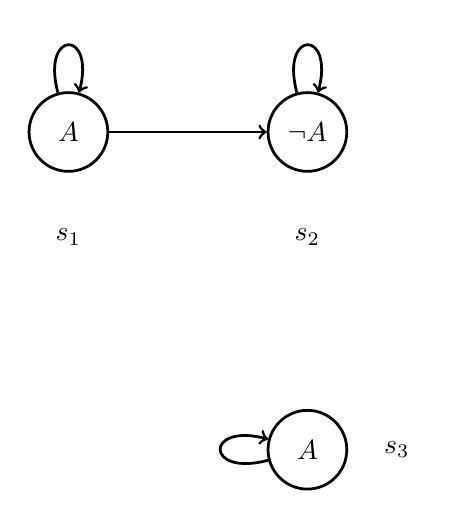
\begin{tikzpicture}[
            node distance=3cm and 2cm,
            every node/.style={draw,circle, minimum size=1cm},
            line width=1pt
        ]
            \node (s1) {$A$};
            \node[right=of s1] (s2) {$\neg A$};
            \node[below=of s2] (s3) {$A$};

            % Accessibility relations
            \draw[->,loop above] (s1) to (s1);     % s1 sees itself
            \draw[->] (s1) -- (s2);                % s1 sees s2
            \draw[->,loop above] (s2) to (s2);     % s2 sees itself
            \draw[->,loop left] (s3) to (s3);      % s3 sees itself

            % Labels
            \node[below=0.3cm of s1,draw=none] {$s_1$};
            \node[below=0.3cm of s2,draw=none] {$s_2$};
            \node[right=0.1cm of s3,draw=none] {$s_3$};
        \end{tikzpicture}
    \end{center}

    \textbf{Conclusion:} modal operators require relational (Kripke) semantics and cannot be captured by truth tables.

    % ---- Exerc 4 ----

    \subsection{Exercise 4}

    Show that the satisfaction of a formula $\varphi$ within a given model is only dependent on the valuation $V$ of the propositional symbols occurring in $\varphi$. In particular, assume that $V$ and $V'$ are two valuations on the frame $(W, R)$ such that $V(p) = V'(p)$ for all symbols $p$ in $\varphi$. Show that
    \[
    (W,R,V) \models \varphi \iff (W,R,V') \models \varphi
    \]
    \emph{Hint: Prove this by induction on the number of connectives in $\varphi$.}

    \textbf{Sketch of proof:}\\
    Proceed by induction on the structure of $\varphi$:
    \begin{itemize}
        \item \emph{Base case:} $\varphi$ is a propositional variable $p$. By assumption $V(p) = V'(p)$, so they agree.
        \item \emph{Inductive steps:}
        \begin{itemize}
            \item If $\varphi = \neg \psi$, use the IH on $\psi$.
            \item If $\varphi = (\psi_1 \wedge \psi_2)$, use IH on $\psi_1, \psi_2$.
            \item If $\varphi = \Box \psi$, by modal semantics: $(W,R,V), w \models \Box \psi$ iff for all $v$ with $wRv$, $(W,R,V), v \models \psi$. By IH, the same applies for $V'$, so satisfaction is preserved.
            \item The same for $\Diamond$ and other connectives.
        \end{itemize}
    \end{itemize}
    Thus, the satisfaction value depends only on the evaluation of the propositional variables that actually occur in the formula.

\end{document}